



The basic software for hypothesis testing on parts of models involves the 
familiar \code{lm} and \code{summary} operators for generating the
regression report and the \code{anova} operator for generating an
\ANOVA\ report on a model.

\subsection{ANOVA reports}


\index{P}{anova@\texttt{anova}}
\index{P}{Hypothesis Testing!anova@\texttt{anova}}

The \code{anova} operator takes a model as an argument and produces
the term-by term \ANOVA\ report.  To illustrate, consider this model
of wages from the Current Population Survey data. \datasetCPS
\begin{Schunk}
\begin{Sinput}
> cps = fetchData("cps.csv")
> mod1 = lm(wage ~ married + age + educ, data=cps)
> anova(mod1)
\end{Sinput}
\begin{Soutput}
Analysis of Variance Table

Response: wage
           Df Sum Sq Mean Sq F value  Pr(>F)    
married     1    142     142    6.74  0.0097 ** 
age         1    338     338   16.02 7.2e-05 ***
educ        1   2399    2399  113.54 < 2e-16 ***
Residuals 530  11197      21                    
---
Signif. codes:  0 '***' 0.001 '**' 0.01 '*' 0.05 '.' 0.1 ' ' 1 
\end{Soutput}
\end{Schunk}

Note the small p-value on the \VN{married} term: \texttt{0.0097}.

To change the order of the terms in the report, you can create a new
model with the explanatory terms listed in a different order.  For
example, here's the \ANOVA~ on the same model, but with \VN{married}
last instead of first:
\begin{Schunk}
\begin{Sinput}
> mod2 = lm(wage ~ age + educ + married, data=cps)
> anova(mod2)
\end{Sinput}
\begin{Soutput}
Analysis of Variance Table

Response: wage
           Df Sum Sq Mean Sq F value  Pr(>F)    
age         1    441     441    20.9 6.1e-06 ***
educ        1   2403    2403   113.7 < 2e-16 ***
married     1     36      36     1.7    0.19    
Residuals 530  11197      21                    
---
Signif. codes:  0 '***' 0.001 '**' 0.01 '*' 0.05 '.' 0.1 ' ' 1 
\end{Soutput}
\end{Schunk}

Now the p-value on \VN{married} is large.  This suggests that much of
the variation in \VN{wage} that is associated with \VN{married} can
also be accounted for by \VN{age} and \VN{educ} instead.


\subsection{Non-Parametric Statistics}

Consider the model of world-record swimming times plotted on page
\pageref{page:interaction-swimming}.  It shows pretty clearly the
interaction between \VN{year} and \VN{sex}.

It's easy to confirm that this interaction term is statistically significant:
\begin{Schunk}
\begin{Sinput}
> swim = fetchData("swim100m.csv")
> anova( lm(time ~ year*sex, data=swim) )
\end{Sinput}
\begin{Soutput}
Analysis of Variance Table

Response: time
          Df Sum Sq Mean Sq F value  Pr(>F)    
year       1   3579    3579   324.7 < 2e-16 ***
sex        1   1484    1484   134.7 < 2e-16 ***
year:sex   1    297     297    26.9 2.8e-06 ***
Residuals 58    639      11                    
---
Signif. codes:  0 '***' 0.001 '**' 0.01 '*' 0.05 '.' 0.1 ' ' 1 
\end{Soutput}
\end{Schunk}

The p-value on the interaction term is very small: $2.8 \times 10^{-6}$.

To check whether this result might be influenced by the shape of the
distribution of the \VN{time} or \VN{year} data, you can conduct a
non-parametric test.  Simply take the rank of each quantitative variable:


\index{C}{non-parametric statistics}
\index{C}{outlier!and non-parametrics}

\index{P}{rank@\texttt{rank}}
\index{P}{Hypothesis Testing!rank@\texttt{rank}}

\begin{Schunk}
\begin{Sinput}
> mod = lm(rank(time) ~ rank(year)*sex, data=swim)
> anova(mod)
\end{Sinput}
\begin{Soutput}
Analysis of Variance Table

Response: rank(time)
               Df Sum Sq Mean Sq F value Pr(>F)    
rank(year)      1  14320   14320 3755.77 <2e-16 ***
sex             1   5313    5313 1393.41 <2e-16 ***
rank(year):sex  1      1       1    0.23   0.63    
Residuals      58    221       4                   
---
Signif. codes:  0 '***' 0.001 '**' 0.01 '*' 0.05 '.' 0.1 ' ' 1 
\end{Soutput}
\end{Schunk}

With the rank-transformed data, the p-value on the interaction term is
much larger: no evidence for an interaction between
\VN{year} and \VN{sex}.  You can see this directly in  a plot of the data
after rank-transforming \VN{time}:

\begin{Schunk}
\begin{Sinput}
> xyplot(rank(time) ~ year, groups=sex, data=swim)
\end{Sinput}
\end{Schunk}
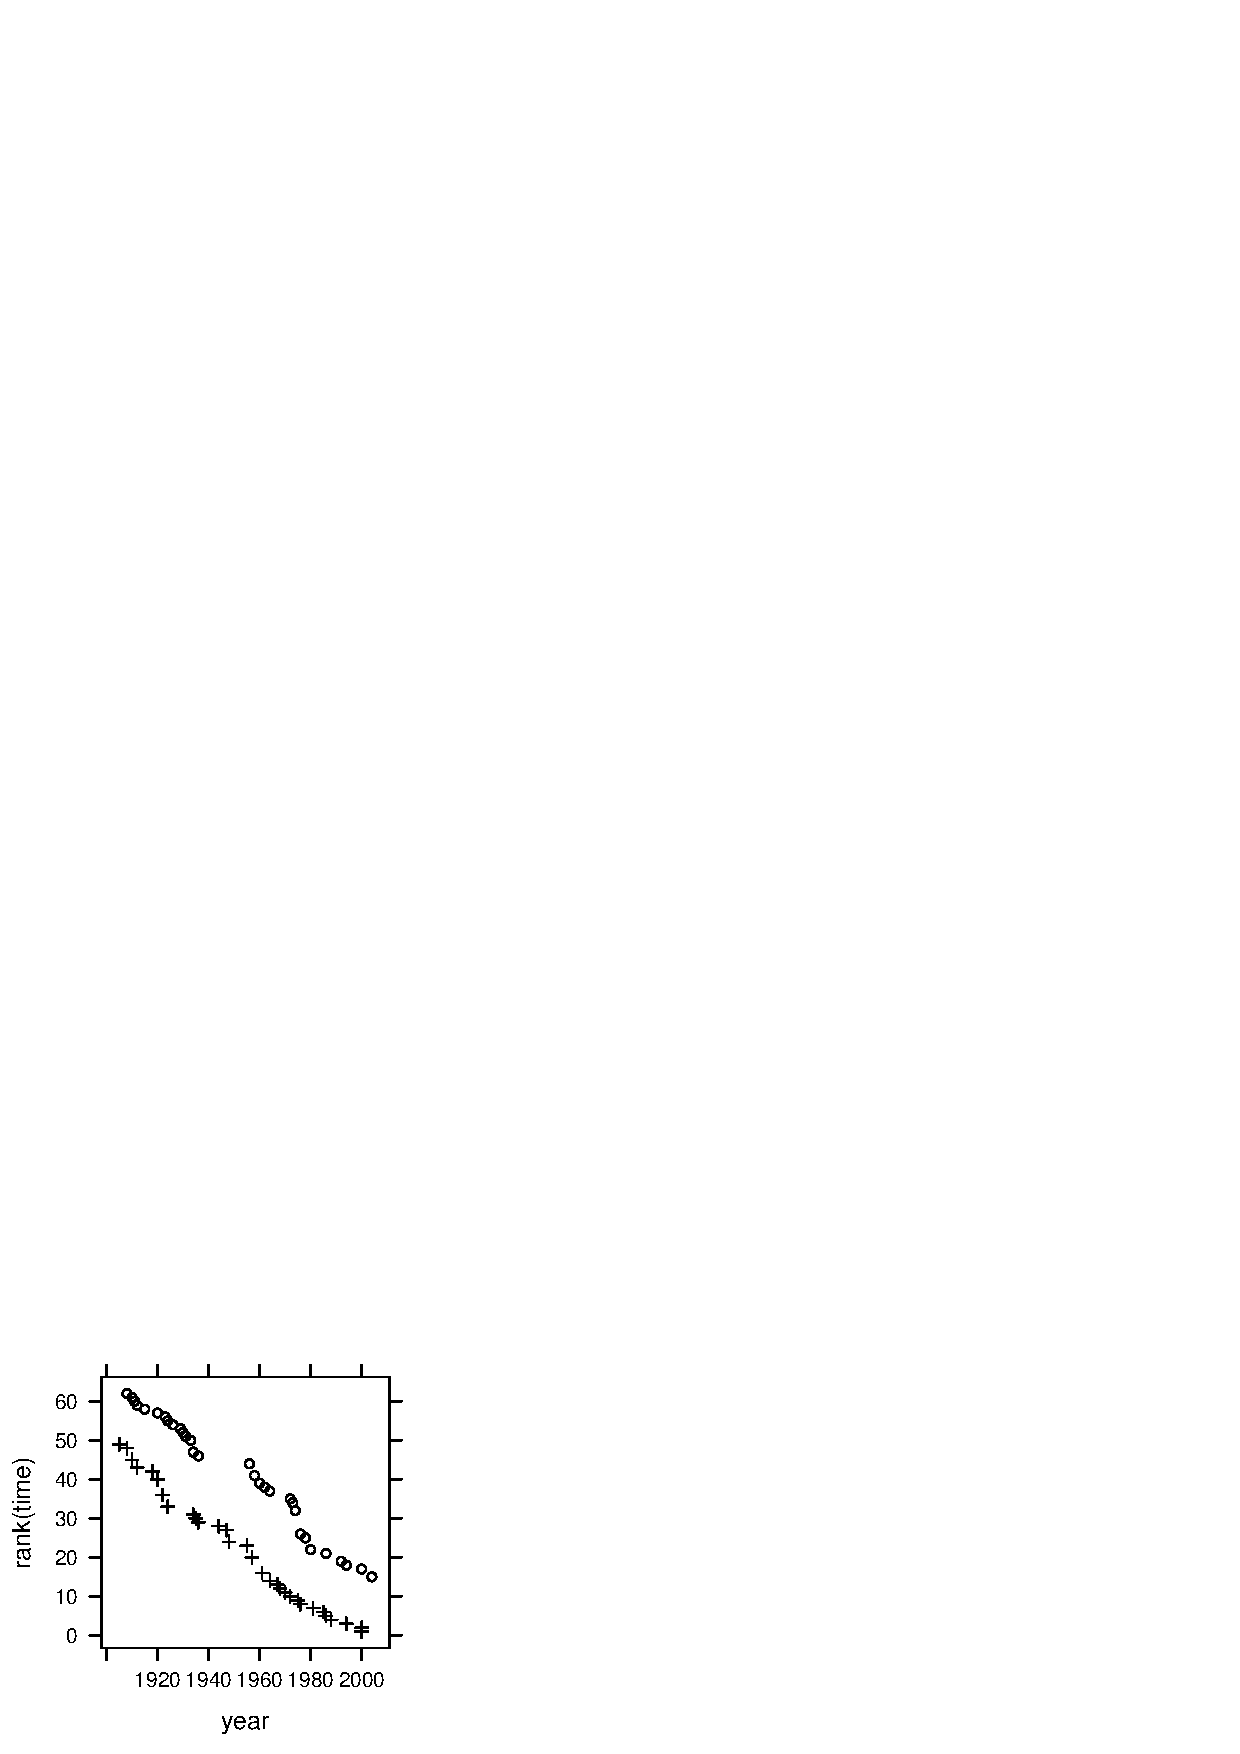
\includegraphics{Figures/traditional-non-param-swim}

The rank-transformed data suggest that women's records are improving
in about the same way as men's.
